\documentclass[a4paper]{report}
% basics
\usepackage{xeCJK}
\setCJKmainfont{Kaiti TC} % 新細明體
\setCJKmainfont{Kaiti TC}[AutoFakeBold=6 , AutoFakeSlant=.2]

\usepackage[letterpaper,top=2cm,bottom=2cm,left=3cm,right=3cm]{geometry}
\linespread{1.2}
\usepackage{amssymb}
\usepackage{amsmath}
\usepackage{graphicx}
\usepackage{amsthm}
\usepackage[dvipsnames]{xcolor}
\usepackage{xeCJK} % 啟用中文支持
\usepackage{circuitikz} % 電路圖
\usepackage{tcolorbox} % 用來加方框
\usepackage{algorithm}
\usepackage[noend]{algpseudocode}
\usepackage{enumitem}
\usepackage{float}
\usepackage{tikz}
\usetikzlibrary{trees}
\usepackage{hyperref}
\usetikzlibrary{arrows.meta,automata,positioning}

% === theorem environments with mdframed ===
\usepackage{thmtools}   % 提供 declaretheorem
\usepackage{mdframed}   % theorem style 加邊框

\declaretheoremstyle[
  headfont=\bfseries\sffamily\color{black}, bodyfont=\normalfont,
  mdframed={
    linewidth=2pt,
    rightline=false, topline=false, bottomline=false,
    linecolor=black,
    nobreak=false
  }
]{thmblueline}

\declaretheorem[style=thmblueline, numbered=no, name=Reason]{reason}

\declaretheoremstyle[
  headfont=\bfseries\sffamily\color{black}, bodyfont=\normalfont,
  mdframed={
    linewidth=2pt,
    rightline=false, topline=false, bottomline=false,
    linecolor=NavyBlue!60!black,
    nobreak=false
  }
]{thmgreenline}

\declaretheorem[style=thmgreenline, numbered=no, name=Note]{note}

\declaretheoremstyle[
  headfont=\bfseries\sffamily\color{red!70!black}, bodyfont=\normalfont,
  mdframed={
    linewidth=2pt,
    rightline=false, topline=false, bottomline=false,
    linecolor=red, backgroundcolor=red!3,
    nobreak=false
  }
]{thmredbox}

\declaretheorem[style=thmredbox, numbered=no, name=Wrong Ans]{wrong}


\declaretheoremstyle[
  headfont=\bfseries\sffamily\color{ForestGreen!70!black}, bodyfont=\normalfont,
  mdframed={
    linewidth=2pt,
    rightline=false, topline=false, bottomline=false,
    linecolor=ForestGreen!70!black, backgroundcolor=ForestGreen!3,
    nobreak=false
  }
]{thmgreenbox}

\declaretheorem[style=thmgreenbox, numbered=no, name=Correct Ans]{cor}

\declaretheoremstyle[
  headfont=\bfseries\sffamily\color{black}, bodyfont=\normalfont,
  mdframed={
    linewidth=2pt,
    linecolor=black,
    nobreak=false
  }
]{thmblackline}

\declaretheorem[style=thmblackline, numbered=no, name=Description]{problem}


\usepackage{titlesec}

\titleformat{\section}
  {\normalfont\Large\bfseries}  % 字型樣式
  {}                            % 不顯示編號
  {0pt}                         % 編號和標題距離
  {Problem\ }                  % 每個 section 都會以 "Problem:" 開頭

\newcommand{\red}[1]{\textcolor{red}{#1}}
\newcommand{\blue}[1]{\textcolor{blue!70!black}{#1}}
\newcommand{\yel}[1]{\textcolor{Goldenrod!70!black}{#1}}
\newcommand{\grn}[1]{\textcolor{ForestGreen!70!black}{#1}}

\newcommand{\yelbox}[1]{%
  {\setlength{\fboxrule}{1pt}%
   \setlength{\fboxsep}{2pt}%
   \color{Goldenrod!90!black}\fbox{\normalcolor #1}}}

\newcommand{\bluebox}[1]{%
  {\setlength{\fboxrule}{1pt}%
   \setlength{\fboxsep}{2pt}%
   \color{cyan!80!black}\fbox{\normalcolor #1}}}

\newcommand{\redbox}[1]{%
  {\setlength{\fboxrule}{1pt}%
   \setlength{\fboxsep}{2pt}%
   \color{red}\fbox{\normalcolor #1}}}

\usepackage{pgfplots}
\pgfplotsset{compat=1.18}

\author{Vinsong}
\title{CSIE7435: Deep Learning Algorithms and Implementations}

\thispagestyle{empty}
\addbibresource{reference.bib}

\usepackage{adjustbox}
\usepackage{centernot}

\begin{document}

\maketitle

\begin{abstract}
    The lecture note of 2025 Fall Deep Learning Algorithms and Implementations by professor 林智仁.
    \vspace{5em}
    \begin{center}
    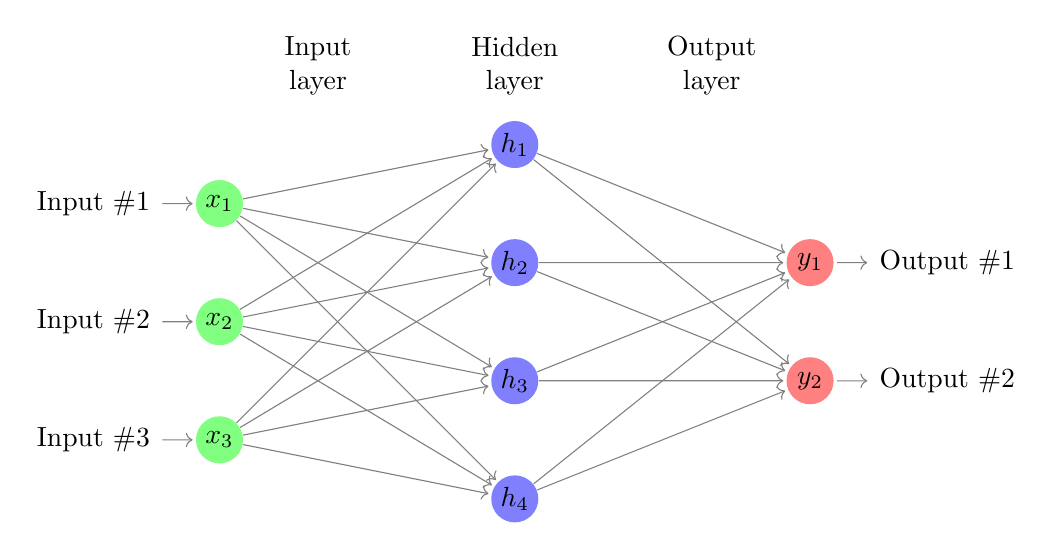
\begin{tikzpicture}[
    % 定義樣式
    shorten >=1pt,->,
    draw=black!50,
    node distance=2.5cm,
    every pin edge/.style={<-,shorten <=1pt},
    neuron/.style={circle,fill=black!25,minimum size=17pt,inner sep=0pt},
    input neuron/.style={neuron, fill=green!50},
    output neuron/.style={neuron, fill=red!50},
    hidden neuron/.style={neuron, fill=blue!50},
    annot/.style={text width=4em, text centered},
    scale=1.5
]

    % 設定各層的數量
    \def\inputNum{3}
    \def\hiddenNum{4}
    \def\outputNum{2}

    % --- 1. 繪製 Input Layer ---
    \foreach \name / \y in {1,...,\inputNum}
        \node[input neuron, pin=left:Input \#\y] (I-\name) at (0,-\y) {$x_{\y}$};

    % --- 2. 繪製 Hidden Layer ---
    % 這裡做了一個位移,讓它稍微置中一點 (視需求調整)
    \foreach \name / \y in {1,...,\hiddenNum}
        \path[yshift=0.5cm]
            node[hidden neuron] (H-\name) at (2.5cm,-\y) {$h_{\y}$};

    % --- 3. 繪製 Output Layer ---
    \foreach \name / \y in {1,...,\outputNum}
        \path[yshift=-0.5cm]
            node[output neuron, pin={[pin edge={->}]right:Output \#\y}] (O-\name) at (5cm,-\y) {$y_{\y}$};

    % --- 4. 連接線 (Edges) ---
    
    % 連接 Input -> Hidden
    \foreach \source in {1,...,\inputNum}
        \foreach \dest in {1,...,\hiddenNum}
            \path (I-\source) edge (H-\dest);

    % 連接 Hidden -> Output
    \foreach \source in {1,...,\hiddenNum}
        \foreach \dest in {1,...,\outputNum}
            \path (H-\source) edge (O-\dest);

    % --- 5. 加上標籤 (Labels) ---
    \node[annot,above of=H-1, node distance=1cm] (hl) {Hidden layer};
    \node[annot,left of=hl] {Input layer};
    \node[annot,right of=hl] {Output layer};

\end{tikzpicture}
    \end{center}
    
    \begin{flushright}
        Vinsong\\
        \today
    \end{flushright}
\end{abstract}


\newpage

\tableofcontents

\setcounter{chapter}{-1}

\lec{1}{50}

\end{document}